\chapter{Modeling}

\section{Introduction to the model} 
 
The engine considered for this thesis work is a 3.6L V6 gasoline engine. The engine needs to be modeled in a mathematical environment in order to understand the relationships between produced work and waste heat generated, and how to develop an effective strategy to reduce the foregoing waste heat and produce additional useful power.

In this case a mathematical model for the mechanical and the thermal behavior of the engine has been developed in MATLAB/Simulink. The model is a backward-looking model, as will be explained in greater detail in Section~\ref{sub:forward_backward}. The model leverages previous models by Professor Marcello Canova and Researcher Luke DeBruin, for reduced development time.
 
\subsection{Inputs and outputs}

In Figure~\ref{fig:model_block_diagram} it's shown the block diagram and conceptual schematic of the model.

\begin{figure}[ht]
  \centering
  \includegraphics[width=\textwidth]{figures/model/block_diagram.pdf}
  \caption{Block diagram of the model\label{fig:model_block_diagram} }
\end{figure}

This model is a \emph{Backward-looking} model, that means that the torque demand is computed from the vehicle speed profile. In Forward-looking models, on the other hand, the vehicle speed is computed from the torque generated by the powertrain. A broader explanation of these two different modeling approaches will be provided in Section~\ref{sub:forward_backward}.
 
\begin{table}[]
  \centering
  \begin{tabular}{ll}
    \hline
    Inputs        & Outputs                                           \\ \hline
    Lock-Up       & Temperature coolant out from the engine block     \\
    Gear          & Temperature oil out from the engine block         \\
    Vehicle speed & Temperature coolant out from the radiator         \\
                  & Heat rejection from the radiator                  \\
                  & Rotational speed at the engine                    \\
                  & Rotational speed at the input of the transmission \\
                  & Fuel mass flow rate                               \\
                  & Torque at the engine                              \\
                  & Torque at the torque converter turbine            \\
                  & Power drawn by the fan                            \\ \hline
  \end{tabular}
  \caption{Inputs and outputs of the engine model\label{tab:inputs_outputs}}
\end{table}

In Table~\ref{tab:inputs_outputs} are shown the inputs and the desired outputs of the model, for both the mechanical an thermal part. The aim of the model is to allow the calculation of the waste heat figures for different driving conditions and engine loads. The vehicle speed is the most important input, because of the backward-looking nature of the model, and it's the starting point for the calculation of the consequent acceleration and torque. The lock-up and gear inputs allows the model to select the correct operational model for the torque converter, and the correct gear ratio in order to calculate rotational speeds in the most precise possible way. The outputs are both thermal and mechanical.

\subsection{Forward and backward modeling approach}
\label{sub:forward_backward}

In general, the approach for writing a model may be of two different kinds: forward-looking or backward-looking. As said before, in a \emph{Forward-looking} model, the vehicle speed is computed from the torque generated by the powertrain. It accounts for  longitudinal vehicle dynamics and effects for crankshaft and transmission inertia, but it's necessary to model the driver behavior, as well as controls for engine, torque converter and transmission. This structure allows to have a very precise model, but may also lead to overly complex and long to develop models.

In a \emph{Backward-looking} model, the torque demand is computed from the vehicle speed profile. In this case, the only information needed are the vehicle speed profile, the torque converter lockup and the gear shift profiles. It does not require detailed information on engine and transmission controls, and the model is quasi-static, hence vehicle longitudinal dynamics and powertrain inertia are neglected. In Figure~\ref{fig:forward_backward_block_diagram} are shown the block diagrams of the structure of a model for both approaches.

\begin{figure}[ht]
  \makebox[\textwidth][c]{\includegraphics[width=1.2\textwidth]{figures/model/forward_backward.pdf}}
  \caption{Block diagram of Powertrain Forward-Looking and Backward-Looking Model\label{fig:forward_backward_block_diagram} }
\end{figure}

The model used in this project is Backward-looking, as the focus of the analysis is on the thermal system and not the complete powertrain. The heat rejection rates from the engine can be calculated easily from this type of model. The effect of coolant, oil and fan cooling on the drive-train efficiency can still be captured by the simulation via the adoption of engine heat rejection maps.

\section{Equations for the mechanical behavior}

The backward model requires inputs and outputs to be inverted with respect to the energy flow in the engine. In this section the equations for the mechanical behavior of the engine will be provided, while in Section~\ref{sec:energy_balance} the energy balance and thermal section of the model will be explained

\subsection{Vehicle Longitudinal Dynamics Model}

The vehicle speed profile is used to calculate the force at wheel, and torque demand at transmission output shaft is calculated from wheel radius and gear ratio.

The force at the wheel may be calculated as:

\begin{equation}
  F_{wheel}=(M+M_{eq})\frac{dV_{veh}}{dt}+F_{aero}+F_{rolling}+F_{grade}
\end{equation}
with the different forces expressed as:

\begin{gather*}
    F_{aero} = C_{s}\rho_{air}\Omega \frac{V^{2}_{veh}}{2} \\
    F_{rolling} = C_{g}M g cos(\Theta) \\
    F_{grade} = 0
\end{gather*}


allows the calculation of the output torque

\begin{equation}
  T_{output}=\frac{F_{wheel}}{R_{wheel}\tau_{diff}}
\end{equation}

\subsection{Transmission model}

Input speed and input torque are computed starting from speed and torque demand at output shaft.

\begin{equation}
  T_{input}=\frac{T_{output}}{\eta(T_{output},\omega_{output})\theta(gear)}
\end{equation}

\begin{equation}
  \omega_{input}=\tau(gear)\omega_{output}
\end{equation}
\subsection{Torque converter model}
To calculate pump speed and torque, the ones relative to the turbine are needed. The Speed ratio may be defined as a function of the turbine speed.

\begin{gather*}
  \omega_{p}    = \frac{\omega_{t}}{SR}             \\
  T_{p}  = \frac{T_{t}}{TR} \\
     \dot{Q_{TC}}  = \omega_{p}T_{p} - \omega_{t}T_{t} 
\end{gather*}

[AGGIUNGI DIAGRAMMI MAPPA SR E TR]

\section{Energy balance}
\label{sec:energy_balance}

This part of the model represents a simplified Thermal Managemet System (TMS) of a typical automotive engine. In Figure~\ref{fig:th_block_diagram} the structure of the model is shown. 

\begin{figure}[ht]
  \centering
  \includegraphics[width=\textwidth]{figures/model/th_block_diagram.pdf}
  \caption{Block diagram of the thermal system model\label{fig:th_block_diagram} }
\end{figure}

This is an engine transient model whose objective is to predict the dynamics of the coolant temperature during warmed conditions, assisting in the design of cooling and oil system thermal control. 

\subsection{Thermal model}

The engine thermal model consists of a lumped parameters thermal mass model that predicts the thermal dynamics of the engine, based on the work of Scott and al. \cite{Scott2012}. Because of the significant differences between coolant and oil temperatures during engine warm up and their effects on engine frcition and coolant temperature, more than one mass is needed. The number of mass selected is three: block, crank, and sump. The \emph{block} contains all the coolant passages and, assuming well mixed coolant, the coolant outlet temperature equals the block average temperature. The \emph{crank} consists of the crankshaft, pistons, connecting rods, main bearings, and supporting structure. The \emph{sump} is the oil reservoir and oil pan structure. In Figure~\ref{fig:engine_mass_scheme} the three masses are shown. The division between the block and the crank is taken at the bottom of the coolant passages. Thus there is both oil and coolant flow to the block but no coolant flow in the crank. The crank-sump division is at the oil pan gasket.

\begin{figure}[ht]
  \centering
  \includegraphics[width=0.8\textwidth]{figures/model/engine_mass_scheme.pdf}
  \caption{Three mass engine model and general engine division into parts\label{fig:engine_mass_scheme} }
\end{figure}

In Figure~\ref{fig:engine_mass_scheme} are shown the energy flows in the engine, according to \cite{Scott2012}. The dotted line represents the boundary used to define the system for the steady state energy balance used in evaluating heat loss to coolant, oil, and convection/radiation. For the engine as a whole, energy enters with fuel and air and leaves with the exhaust gas, brake power, and heat rejected to coolant, oil, and surrounding ambient. At steady state, the energy flows must balance.

\begin{figure}[ht]
  \centering
  \includegraphics[width=0.5\textwidth]{figures/model/energy_flows.pdf}
  \caption{Energy flows in the engines\label{fig:energy_flows} }
\end{figure}

The gross indicated mechanical power released by the combustion process minus the pumping work is the net indicated mechanical power that acts on the piston face, shown as $W_{ni}$ in the diagram. The pumping word in converted to heat and, plus the heat from the combustion, is transferred to the cylinder walls, head, and piston. The heat energy that enters the engine can be calculated from the energy balance on the combustion chamber.

\begin{equation}
  \dot{Q}_{heat} = \dot{E}_{air}+\dot{E}_{fuel}-\dot{E}_{ex}-\dot{W}_{ni}
\end{equation}

The friction power may be determined, is direct measures of indicated power and pumping work are available, as:

\begin{equation}
  \dot{W}_{f}=\dot{W}_{ni}-\dot{W}_{b}
\end{equation}

$Q_{heat}$ and $W_{f}$ may be determined from steady state tests on the engine. Correlating then them with engine operating parameters, for any required brake power and RPM it's possible to find $Q_{heat}$ and $W_{f}$ for use.

The energy flows needs thus to divided among the three thermal masses. The friction work may be divided between the crank, which includes the pistons, and the block, which includes the valve train. $f_{v}$ can be defined as the fraction of the total friction work that is assigned to the block mass. The heat leaving the combustion process goes to the block and the piston, then it's possible to define $f_{h}$ as the fraction of $Q_{heat}$ that goes to the block.

The energy transfers between the block, crank, and sump take place through the conduction paths and the oil flow. The conduction between the masses is considered to be a linear function of the temperature differences, using an overall heat transfer coefficient $UA_{bc}$ between the block and the crank, and $UA_{cs}$ between the crank and the sump. Each mass has some thermal capacity C equal to mass times specific heat.

The transient heat equations for the three engine thermal maps are now shown:

\uline{BLOCK MASS}


\begin{equation}
  \begin{split}
    C_{b}\frac{dT_{b}}{dt}  = &f_{h}\dot{Q}_{heat} + f_{v}\dot{W}_f - f_b\dot{m}_oc_{po}[T_b-T_c]  - UA_{bc}[T_b-T_c] \\
    &- UA_{ba}[T_b-T_a] - \dot{m}_cc_{pc}[T_b-T_{ci}]
  \end{split}
\end{equation}

\uline{CRANK MASS}

\begin{equation}
  \begin{split}
    C_c \frac{dT_c}{dt} = &[1-f_h]\dot{Q}_{heat} + [1-f_v]\dot{W}_f + UA_{bc}[T_b-T_c]-f_b\dot{m}_oc_{cpo}[T_c-T_b] \\
    &+\dot{m}_oc_{po}[T_s-T_c] - UA_{cs}[T_c-T_s] - UA_{ca}[T_c-T_a]
  \end{split}
\end{equation}

\uline{SUMP MASS}

\begin{equation}
  C_s \frac{dT_s}{dt} = \dot{m}_oc_{po}[T_c-T_s]+UA_{cs}[T_c-T_s]-UA_{sa}[T_s-T_a]
\end{equation}


\subsection{Radiator model}

The radiator has a relatively slow response, due to the large thermal mass. The model is based on a paper by Scott and al.~\cite{Scott2003}, and it's a simplified version of the multi-node thermal model. Only one node is considered, and three different energy balance equations has to be defined.

\uline{Energy Balance for COOLANT CONTROL VOLUME}

\begin{equation}
  C_c \frac{dT_c}{dt} = \dot{m}_cc_{p,c}(T_{c,in}-T_c)-A_f \frac{C_f\dot{m}_c^\beta}{C_3}(T_c-T_w)
\end{equation}

\uline{Energy balance for WALL THERMAL MASS}

\begin{equation}
  C_w  \frac{dT_w}{dt} = A_f \frac{C_f\dot{m}_c^\beta}{C_3}(T_c-T_w) - A_f \frac{1}{C_2}(T_w-T_s)
\end{equation}

\uline{Energy balance for FINS AND EXTERNAL SURFACE IN CONTACT WITH AIR}

\begin{equation}
  C_w  \frac{dT_s}{dt} = A_f \frac{1}{C_2}(T_w-T_s) - A_f \frac{(\rho_{air}V_{face})^\frac{2}{3}}{C_1}(T_s-T_{air})
\end{equation}

In steady-state conditions, the heat transfer through the radiator assumes the simplified formulation

\begin{equation}
  \begin{split}
    \dot{Q} &= A_f \frac{C_f\dot{m}_c^\beta}{C_3}(T_c-T_w) \\ &= A_f \frac{1}{C_2}(T_w-T_s) \\ &= A_f \frac{(\rho_{air}V_{face})^{\frac{2}{3}}}{C_1}(T_s-T_{air})
  \end{split}
\end{equation}


\section{Results}

In this sections the results of the model will be presented and explained. Two different drive-cycles have been used to test the model in different conditions and on different use cases. The drive-cycles considered are the \emph{New European Drive Cycle} (NEDC), which is supposed to represent the typical usage of a car in Europe, and \emph{Federal Test Procedure 75} (FTP-75), which is a test procedure defined by the US Environmental protection agency and more representative of US car usage. The standard speed profiles for both drive cycles are shown in Figure~\ref{fig:speed_profile}

\begin{figure}[ht]
  \centering
  \begin{subfigure}[b]{0.45\textwidth}
    \includegraphics[width=\textwidth]{figures/model/NEDC_plt_speed.png}
    \caption{NEDC}
    \label{fig:NEDC_speed_profile}
  \end{subfigure}
  ~ %add desired spacing between images, e. g. ~, \quad, \qquad, \hfill etc. 
  % (or a blank line to force the subfigure onto a new line)
  \begin{subfigure}[b]{0.45\textwidth}
    \includegraphics[width=\textwidth]{figures/model/FTP_plt_speed.png}
    \caption{FTP}
    \label{fig:FTP_speed_profile}
  \end{subfigure}
  \caption{Speed profiles of the considered drivecycles}\label{fig:speed_profile}
\end{figure}

As explained in Section~\ref{sub:forward_backward}, being the model Backward-looking, the gear shifting data and lockup status for the torque converter must be provided from direct measurements on the vehicle. Figure~\ref{fig:lockup} shows the aforementioned data needed for running the simulation.

\begin{figure}[ht]
  \centering
  \begin{subfigure}[b]{0.45\textwidth}
    \includegraphics[width=\textwidth]{figures/model/NEDC_plt_lockup.png}
    \caption{NEDC}
    \label{fig:NEDC_lockup}
  \end{subfigure}
  ~ %add desired spacing between images, e. g. ~, \quad, \qquad, \hfill etc. 
  % (or a blank line to force the subfigure onto a new line)
  \begin{subfigure}[b]{0.45\textwidth}
    \includegraphics[width=\textwidth]{figures/model/FTP_plt_lockup.png}
    \caption{FTP}
    \label{fig:FTP_lockup}
  \end{subfigure}
  ~
  \begin{subfigure}[b]{0.45\textwidth}
    \includegraphics[width=\textwidth]{figures/model/NEDC_plt_gear.png}
    \caption{NEDC}
    \label{fig:NEDC_gear}
  \end{subfigure}
  ~ %add desired spacing between images, e. g. ~, \quad, \qquad, \hfill etc. 
  % (or a blank line to force the subfigure onto a new line)
  \begin{subfigure}[b]{0.45\textwidth}
    \includegraphics[width=\textwidth]{figures/model/FTP_plt_gear.png}
    \caption{FTP}
    \label{fig:FTP_gear}
  \end{subfigure}
  \caption{Lockup and gear profiles}\label{fig:lockup}
\end{figure}

The first mechanical parameter that the model calulates

\begin{figure}[ht]
  \centering
  \begin{subfigure}[b]{0.45\textwidth}
    \includegraphics[width=\textwidth]{figures/model/NEDC_plt_w_trans_in.png}
    \caption{NEDC}
    \label{fig:NEDC_w_trans_in}
  \end{subfigure}
  ~ %add desired spacing between images, e. g. ~, \quad, \qquad, \hfill etc. 
  % (or a blank line to force the subfigure onto a new line)
  \begin{subfigure}[b]{0.45\textwidth}
    \includegraphics[width=\textwidth]{figures/model/FTP_plt_w_trans_in.png}
    \caption{FTP}
    \label{fig:FTP_w_trans_in}
  \end{subfigure}
  \caption{Rotational speed at transmission input}\label{fig:w_trans_in}
\end{figure}

\begin{figure}[ht]
  \centering
  \begin{subfigure}[b]{0.45\textwidth}
    \includegraphics[width=\textwidth]{figures/model/NEDC_plt_w_engine.png}
    \caption{NEDC}
    \label{fig:NEDC_w_engine}
  \end{subfigure}
  ~ %add desired spacing between images, e. g. ~, \quad, \qquad, \hfill etc. 
  % (or a blank line to force the subfigure onto a new line)
  \begin{subfigure}[b]{0.45\textwidth}
    \includegraphics[width=\textwidth]{figures/model/FTP_plt_w_engine.png}
    \caption{FTP}
    \label{fig:FTP_w_engine}
  \end{subfigure}
  \caption{Rotational speed at the engine}\label{fig:w_engine}
\end{figure}

\begin{figure}[ht]
  \centering
  \begin{subfigure}[b]{0.45\textwidth}
    \includegraphics[width=\textwidth]{figures/model/NEDC_plt_T_engine.png}
    \caption{NEDC}
    \label{fig:NEDC_T_engine}
  \end{subfigure}
  ~ %add desired spacing between images, e. g. ~, \quad, \qquad, \hfill etc. 
  % (or a blank line to force the subfigure onto a new line)
  \begin{subfigure}[b]{0.45\textwidth}
    \includegraphics[width=\textwidth]{figures/model/FTP_plt_T_engine.png}
    \caption{FTP}
    \label{fig:FTP_T_engine}
  \end{subfigure}
  \caption{Engine torque}\label{fig:T_engine}
\end{figure}

\begin{figure}[ht]
  \centering
  \begin{subfigure}[b]{0.45\textwidth}
    \includegraphics[width=\textwidth]{figures/model/NEDC_plt_m_dot_f.png}
    \caption{NEDC}
    \label{fig:NEDC_m_dot_fuel}
  \end{subfigure}
  ~ %add desired spacing between images, e. g. ~, \quad, \qquad, \hfill etc. 
  % (or a blank line to force the subfigure onto a new line)
  \begin{subfigure}[b]{0.45\textwidth}
    \includegraphics[width=\textwidth]{figures/model/FTP_plt_m_dot_f.png}
    \caption{FTP}
    \label{fig:FTP_m_dot_fuel}
  \end{subfigure}
  \caption{Fuel mass flow rate}\label{fig:m_dot_fuel}
\end{figure}

\begin{table}[]
  \centering
  \begin{tabular}{lll}
    \hline
    Variable               & NRMSE  & NMSE   \\ \hline
    $\omega$ in transmission & 0.7859 & 0.9542 \\
    $\omega$ engine          & 0.3651 & 0.5969 \\
    T engine               & 0.2797 & 0.4812 \\
    $\dot{m}$ fuel           & 0.5947 & 0.8357 \\ \hline
  \end{tabular}
  \caption{Accuracy of simulation for the mechanical model}
  \label{tab:accuracy_mechanical}
\end{table}

\begin{figure}[ht]
  \centering
  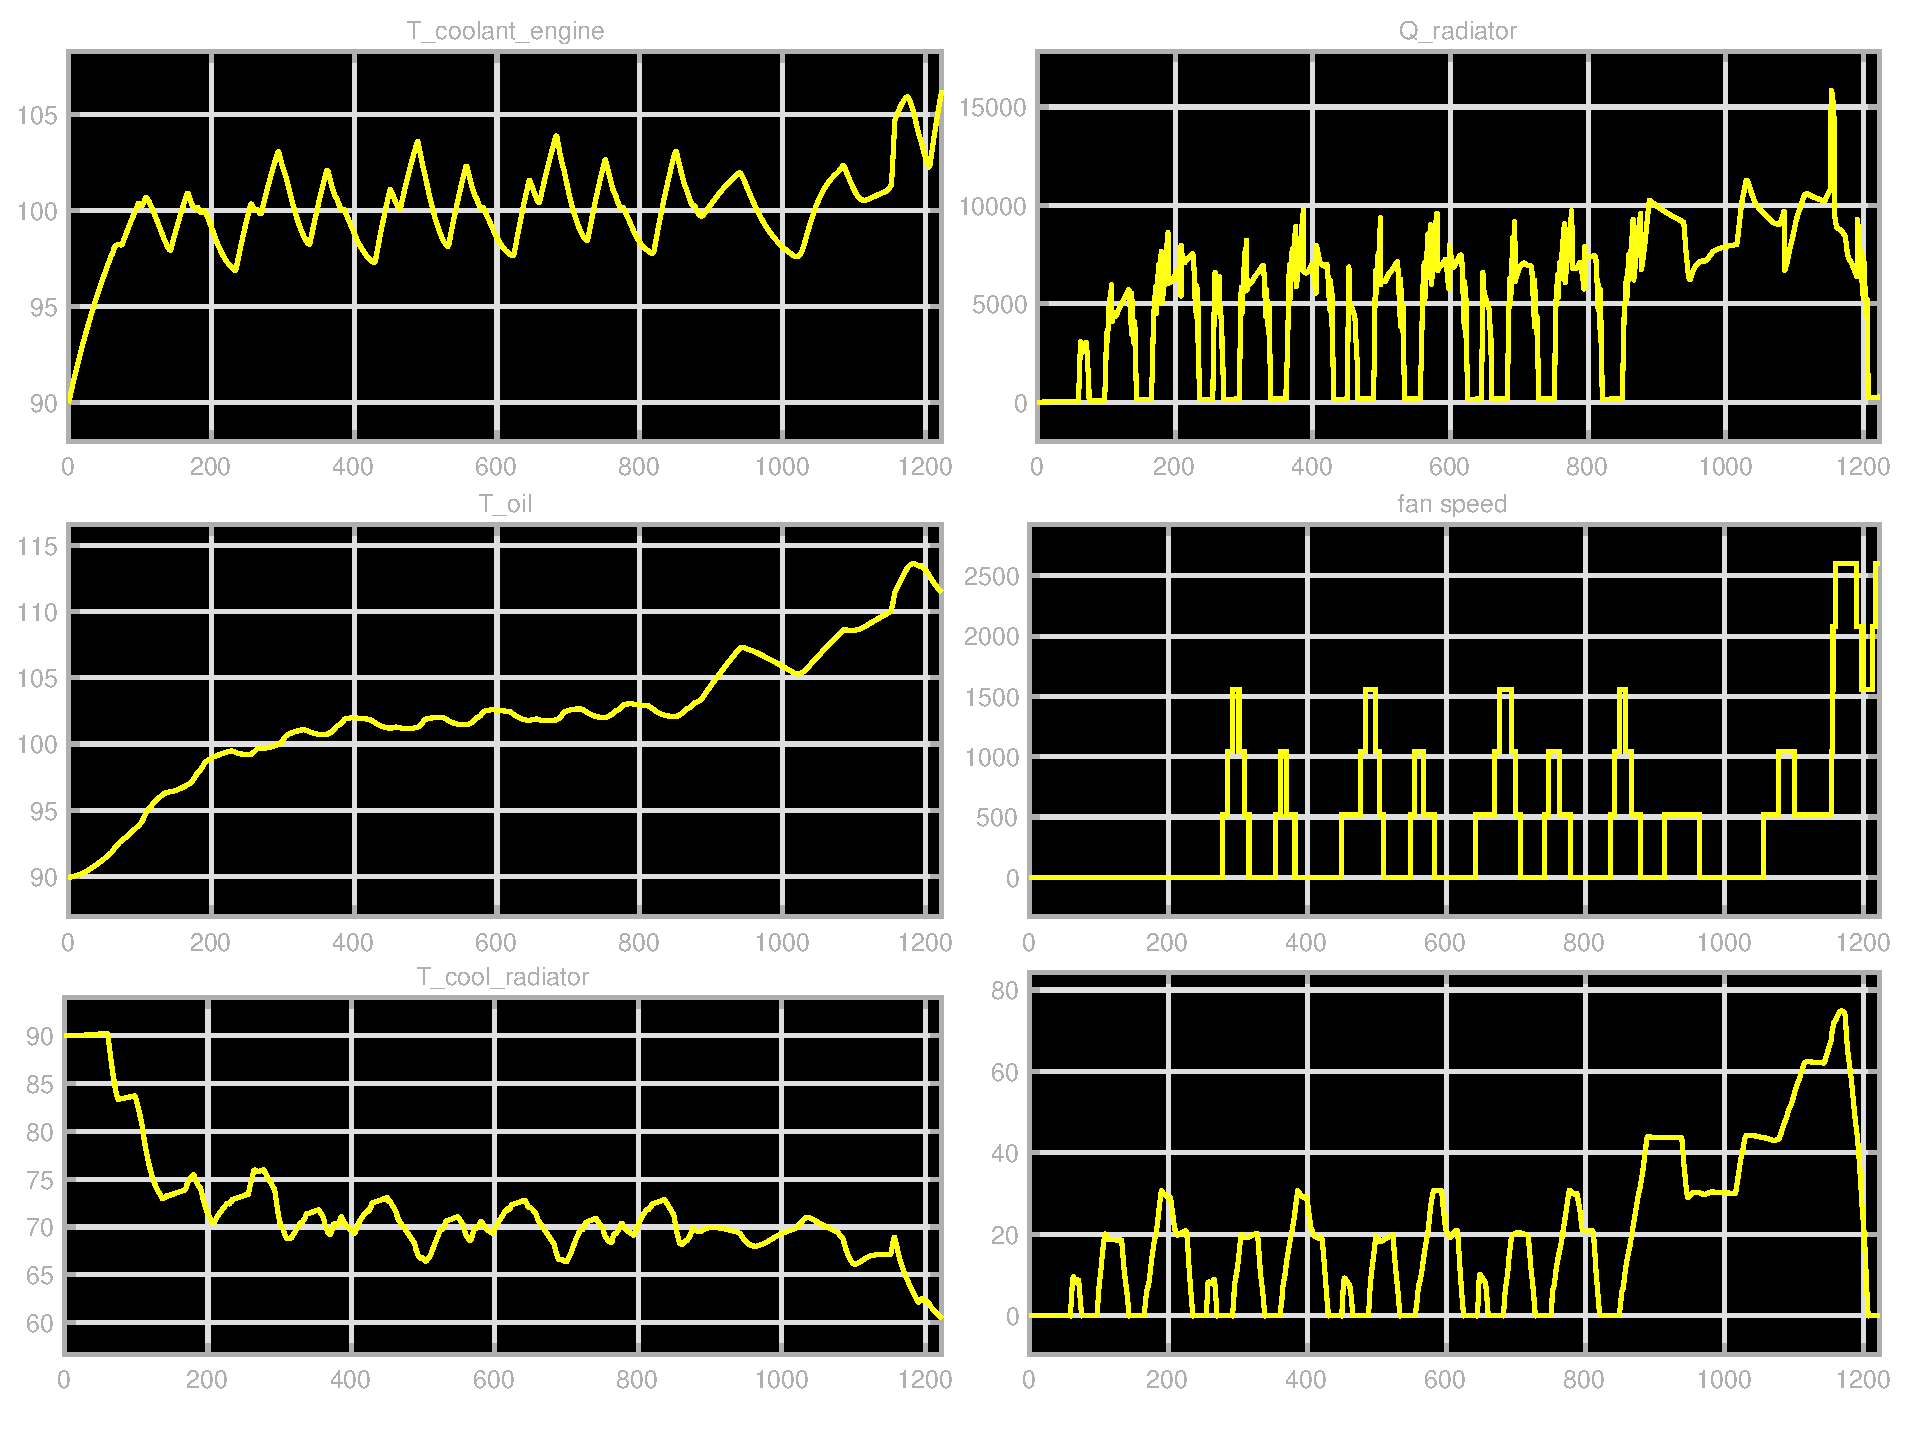
\includegraphics[width=\textwidth]{figures/model/th_results_NEDC.eps}
  \caption{Thermal model results for New European Driving Cycle\label{fig:th_results_NEDC} }
\end{figure}

\begin{figure}[ht]
  \centering
  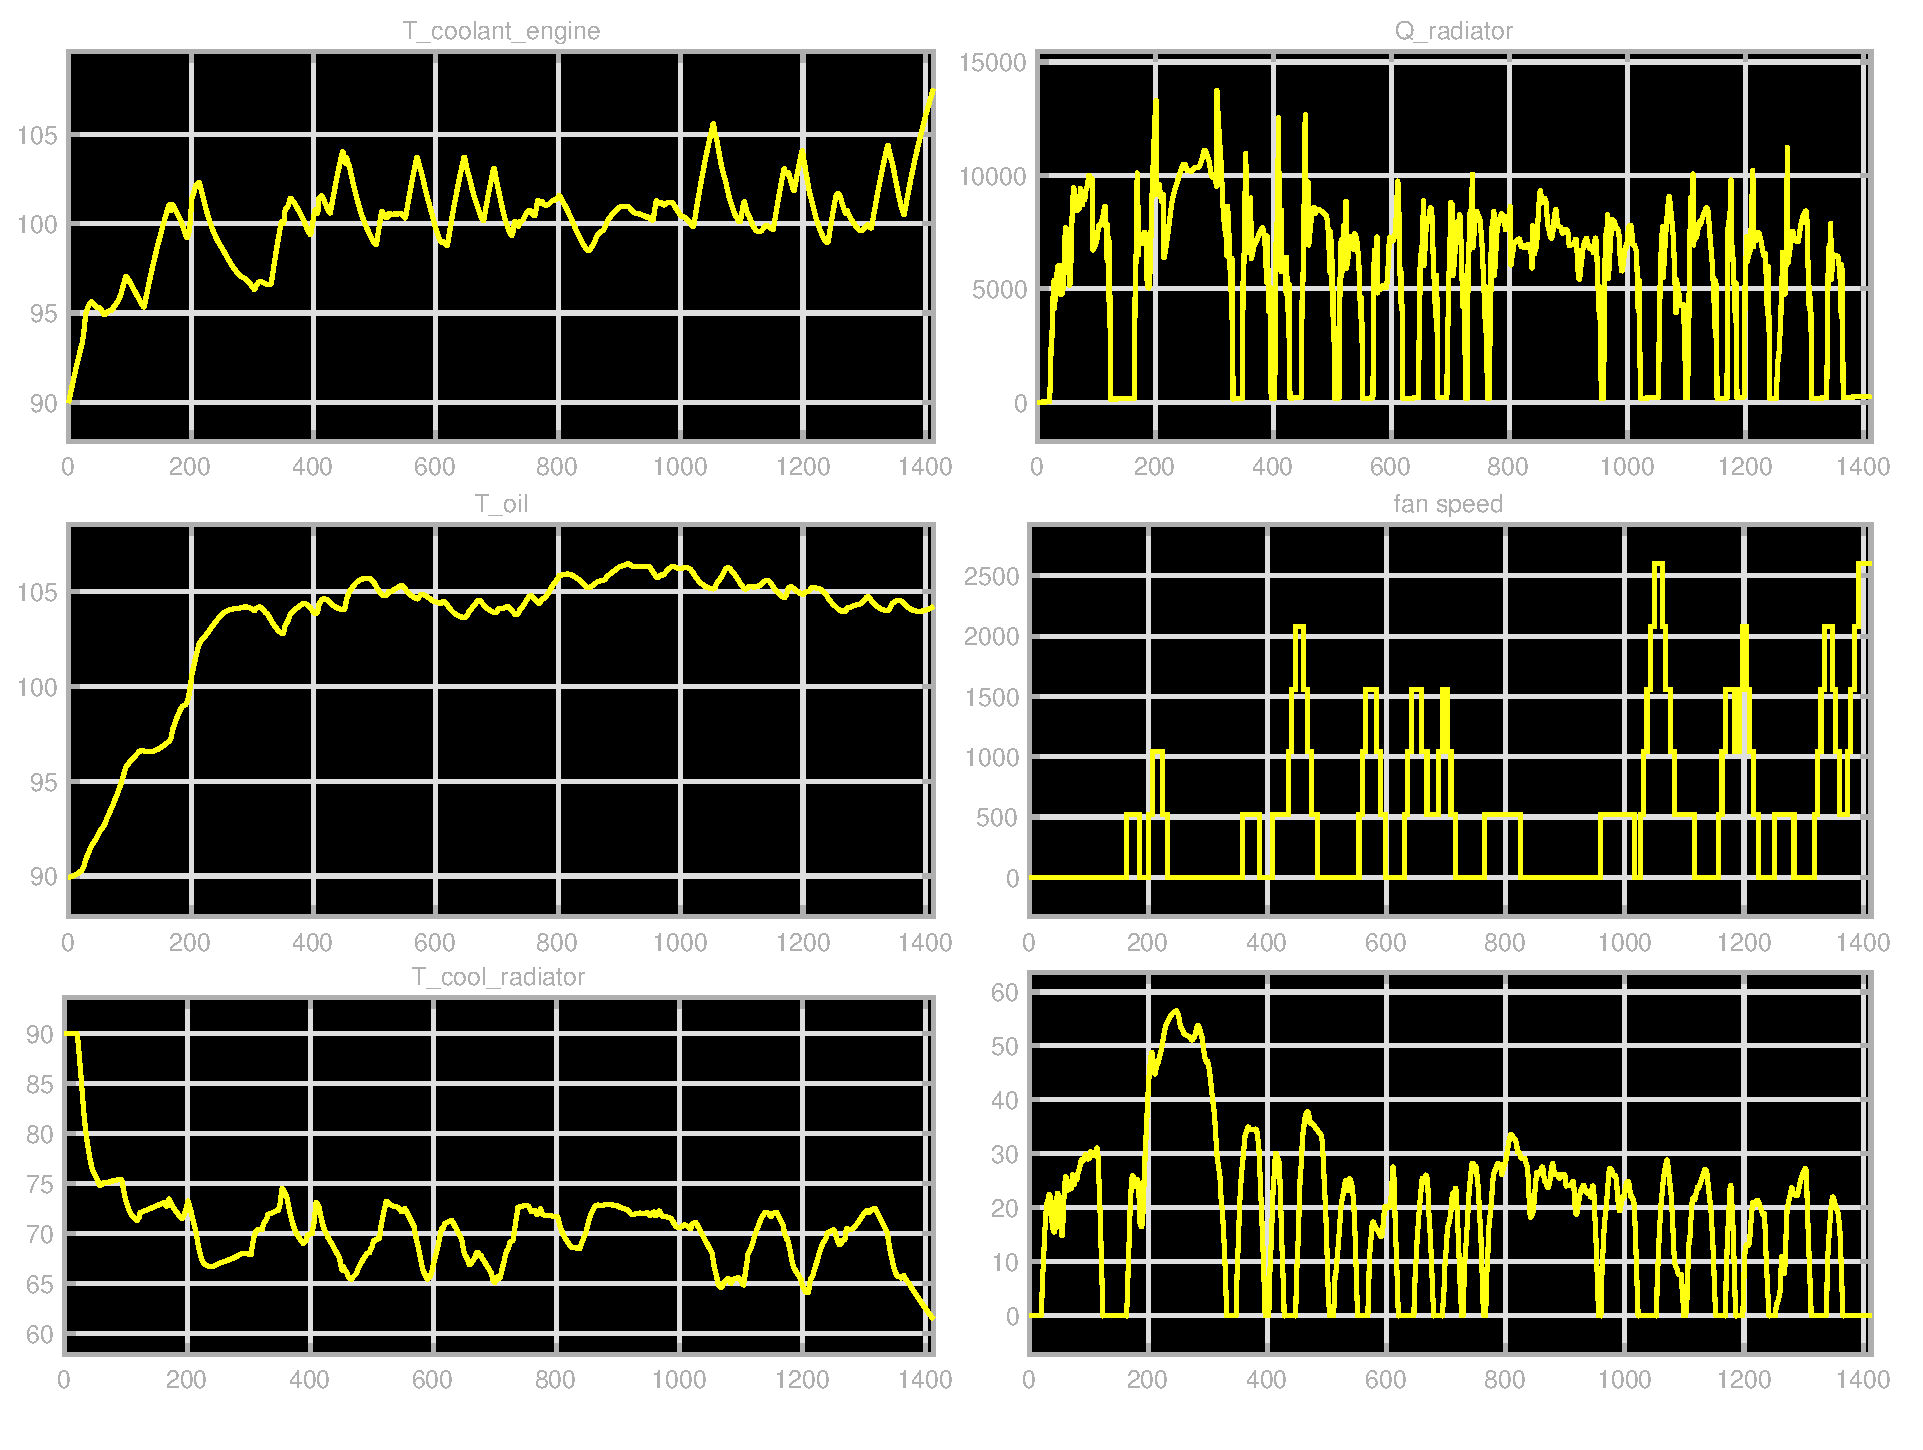
\includegraphics[width=\textwidth]{figures/model/th_results_FTP.eps}
  \caption{Thermal model results for Federal Test Procedure 75\label{fig:th_results_FTP} }
\end{figure}
~

%%% Local Variables:
%%% mode: latex
%%% TeX-master: "thesis"
%%% End:
